\documentclass{beamer}
\usepackage[left=1.2in,right=1in,top=1in,bottom=1in]{geometry}
\usepackage[romanian]{babel}
\usepackage[T1]{fontenc}
\usepackage{unicode-math}
\usepackage{minted}
\usepackage{listings}
\usepackage{color}
\title{Verificare Formală}
\author{Amza Rareș, Dienes Oliviu, Militaru Oana}
\institute{Universitatea de Vest din Timișoara\\
Facultatea de Matematică și Informatică, Inginerie Software}

\begin{document}

\begin{frame}
  \titlepage
  \begin{figure}
    \centering
    
\includegraphics[width=0.3\textwidth]{Logo-UVT.png}
  \end{figure}
\end{frame}

\begin{frame}
  \frametitle{Cuprins}
  \tableofcontents
\end{frame}

\section{Descriere Dataset }
\begin{frame}
  \frametitle{}
    Datasetul ACAS XU este conceput pentru a evalua performanța sistemului de
    evitare a coliziunilor integrate (ACAS Xu) și de detectare și evitare (DAA) în cazul sistemelor de aviație cu asistență la distanță (UAS). \cite{acasxu-github}
  Informații despre acest dataset:  

\end{frame}
\subsection{Tipul de rețea}
\begin{frame}
  \frametitle{Tipul de rețea}
  Modelul ACAS XU este o rețea complet conectată (Fully Connected - FC).
  Funcția de activare folosită este ReLU. \cite{deepai-relu} %\cite{nasareport}
\end{frame}

\subsection{Rețea complet conectată (Fully Connected - FC)}
\begin{frame}
  \frametitle{Rețea complet conectată (Fully Connected - FC)}

  O rețea complet conectată este un tip de arhitectură neuronală în care fiecare neuron dintr-un strat este conectat la fiecare neuron din stratul următor.
  În cazul modelului ACAS XU, aceasta înseamnă că toți cei 5 neuroni de intrare sunt conectați la toți cei 13.000 de neuroni din stratul următor.
  Acest tip de arhitectură este utilizat într-o varietate de aplicații și permite modelului să învețe relații complexe între datele de intrare. \cite{arxiv2022} \cite{ieee2019} \cite{springer-chapter}
\end{frame}

\subsection{Funcția de activare ReLU (Rectified Linear Unit)}
\begin{frame}
  \frametitle{Funcția de activare ReLU (Rectified Linear Unit)}

  ReLU este o funcție de activare comună folosită în rețelele neuronale. Ea returnează 0 pentru toate valorile negative și returnează valoarea de intrare pentru valorile pozitive.
  Această funcție de activare adaugă non-linearitate modelului, ceea ce îi permite să învețe și să captureze relații complexe în date. \cite{deepai-relu} \cite{arxiv-1803.08375}
\end{frame}

\subsection{Numărul de parametrii}
\begin{frame}
  \frametitle{Numărul de parametrii}

  Modelul ACAS XU are 13.000 de parametrii. Acești parametrii reprezintă ponderile și bias-urile asociate cu conexiunile dintre neuroni și permit modelului să învețe de la datele de antrenare. \cite{ieee2019}
\end{frame}

\subsection{Dimensiunea de intrare}
\begin{frame}
  \frametitle{Dimensiunea de intrare}

  Dimensiunea de intrare a modelului ACAS XU este 5, ceea ce înseamnă că modelul primește un vector de 5 elemente ca intrare pentru fiecare exemplu de date. \cite{nasa}
\end{frame}

\subsection{Raritatea (Sparsity)}
\begin{frame}
  \frametitle{Raritatea (Sparsity)}

  Raritatea modelului ACAS XU variază între 0\% și 20\%. Acest lucru poate să se refere la proporția de conexiuni care au ponderi nenule față de totalul conexiunilor posibile.
\end{frame}
\begin{frame}
  \frametitle{}
Algoritmul folosește o rețea neuronală profundă (DNN) pentru comprimarea unei tabele numerice mari care conține scoruri asociate cu diferite manevre din milioane de stări discrete. Această rețea neurală profundă are 128 straturi, dintre care 5-128-64-32-16-5 și 5-256-128-64-32-16-5. Funcțiile activate folosite sunt funcții sigure standard (ReLU) sau funcții sigure saturate (Leaky ReLU). Numărul total de parametri ale rețelei neurali profundă este estimat la aproximativ 1.6 milioane. \cite{nasa2018} \cite{arxiv2018}
\end{frame}



\section{Instalare Instrumente}
\begin{frame}
  \frametitle{Instalare Instrumente}
{\( \alpha \),\( \beta \)-CROWN (alpha-beta-crown)} este un verificator de rețele neuronale care a câștigat competiția VNN-COMP 2021, 2022 și 2023
având cel mai mare scor total și astfel depășind în performanță multe alte verificatoare de rețele neuronale pe o gamă largă de evaluări în decursul a 2 ani. \cite{alpha-beta-crown}
Acesta este un instrument care funcționează doar în sistemul de operare Linux. 

Înainte de a începe configurarea instrumentului trebuie să verificăm dacă avem git și Miniconda instalate, iar în caz contrar să le instalăm urmând link-urile unde se găsesc fișierele pentru instalare: https://git-scm.com și https://docs.conda.io/projects/miniconda/en/latest/.

\item După setarea mediului de lucru vom accesa pagina unde se află proiectul (https://github.com/Verified-Intelligence/alpha-beta-CROWN) și vom urma pașii indicați.

\end{frame}

\begin{frame}[containsverbatim]
  %\frametitle{Instalare Instrumente}
Deoarece am lucrat pe o mașină cu sistemul Windows toate comenzile ulterioare au fost efectuate cu ajutorul WSL și Ubuntu și am urmat următorii pași pentru a configura proiectul:
    \item 1. Am clonat proiectul pe dispozitivul nostru cu comanda git clone 
    \begin{minted}{shell}
    git clone --recursive https://github.com
    /Verified-Intelligence/alpha-beta-CROWN.git
    \end{minted}
    \item 2. Am creat mediul de lucru din Conda :
    \begin{minted}{shell}
    conda env create -f /complete_verifier
    /environment_pyt111.yaml --name alpha-beta-crown
    \end{minted}
    
\end{frame}
\begin{frame}[containsverbatim]
  %\frametitle{Instalare Instrumente}
  
  \item 3. După ce au fost instalate toate modulele necesare vom verifica că mediul de lucru a fost creat.
        \begin{figure}[!h]
          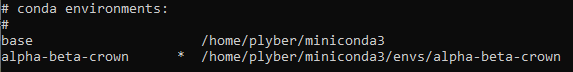
\includegraphics[width=\linewidth]{1condaenvs.PNG}
          \caption{Verificare mediu de lucru Conda}
          \label{fig:mediilucruconda}
        \end{figure}
        
    \item 4. Pentru a putea folosi verificatorul trebuie să configurăm și submodulul auto\_LiRPA: 
     \begin{minted}{shell}
    cd auto_LiRPA
    python setup.py install
    \end{minted}
\end{frame}

\begin{frame}[containsverbatim]
  \frametitle{Rulare Instrumente pentru Benchmark}
  Fiind cu două directoare deasupra complete\_verifier, am clonat repository-ul vnncomp2023\_benchmarks\cite{vnncomp2023_benchmarks} astfel încât calea specificată în fișierul de tip yaml să coincidă cu calea necesară pentru funcționarea instrumentului \( \alpha \),\( \beta \)-CROWN:
    \begin{minted}{shell}
    ../../vnncomp2023_benchmarks/benchmarks/acasxu
    \end{minted}
    Ne-am asigurat că am activat mediul de lucru ab-crown cu Miniconda3 folosind următoarea instrucțiune: 
    \begin{minted}{shell}
    conda activate alpha-beta-crown
    \end{minted}
    Apoi am rulat abcrown.py pe benchmarkul acasxu.yaml:
    \begin{minted}{shell}
    cd complete_verifier
    python abcrown.py --config exp_configs/acasxu.yaml
    \end{minted}

\end{frame}

\begin{frame}[containsverbatim]
    %\frametitle{Rulare Instrumente pentru Benchmark}
Execuția instrumentului s-a finalizat cu succes și am primit următoarele rezultate:
    \begin{minted}{shell}
############# Summary #############
Final verified acc: 74.19354838709677% (total 186 examples)
Problem instances count: 186 ,
total verified (safe/unsat): 138 ,
total falsified (unsafe/sat): 47 ,
timeout: 1
mean time for ALL instances (total 186):3.258072501031987,
max time: 118.92911696434021

    \end{minted}
    Astfel avem o acuratețe finală de 74,19\% pentru 186 de instanțe: 138 instanțe fiind SAT și 47 UNSAT. De asemenea, una dintre instanțe a depășit timpul alocat, astfel că am avut și un timeout.

\end{frame}

\section{Bibliografie}
\begin{frame}[allowframebreaks]
  \frametitle{Bibliografie}
\begin{enumerate}
\bibliographystyle{IEEEtran}
\bibliography{IEEEabrv, mybib}
%\addcontentsline{toc}{chapter}{Bibliografie}
\end{enumerate}
\end{frame}

\end{document}

